\part{Annexe}
\begin{frame}[noframenumbering]{Annexe}
\begin{multicols}{2}
\tableofcontents
\end{multicols}
\end{frame}

\section{Annexe Mckay}
\subsection{Arbre de recherche}
\begin{frame}[noframenumbering]{Arbre de recherche de permutations}
    \begin{minipage}{0.3\textwidth}
        \begin{figure}[!htb]
            \centering
            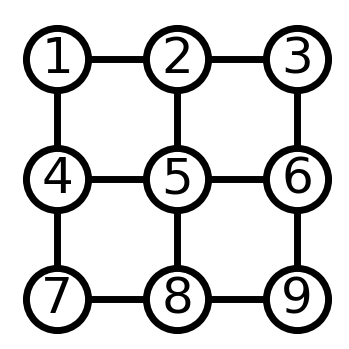
\includegraphics[width = 1.7cm]{graph_tri_equal}
            \caption{\label{fig: Graph G2}Graph G}
        \end{figure}
    \end{minipage}
    \begin{minipage}{0.6\textwidth}
        \begin{center}
            On considère le tri suivant le degré :\newline
            $\pi = (1\ 3\ 7\ 9\ |\ 2\ 4\ 6\ 8\ |\ 5)\qquad $ \newline \newline
            $R(\pi)=\pi$ est alors la racine de l'arbre
        \end{center}
    \end{minipage}
    \newline \newline \newline
    \underline{Trouver les fils} :
    \begin{itemize}
        \item trouver la première partie $V_i$ d'au moins 2 éléments de $\pi$
        \item pour $v \in V$, on crée \textbf{artificiellement} un nouveau tri équitable :
        $\quad \longrightarrow \quad \pi_v = \pi \perp v = R(\ (V_1|..|\ \lbrace v \rbrace \ |\ V_i \textbackslash \lbrace v \rbrace\ |..)\ )$
        \item chacun des tris créés est un fils, on réitère jusqu'à obtenir des tris triviaux (paquets de taille 1)
    \end{itemize}
\end{frame}

\begin{frame}[noframenumbering]{Arbre de recherche de permutations}
    \begin{figure}[!htb]
        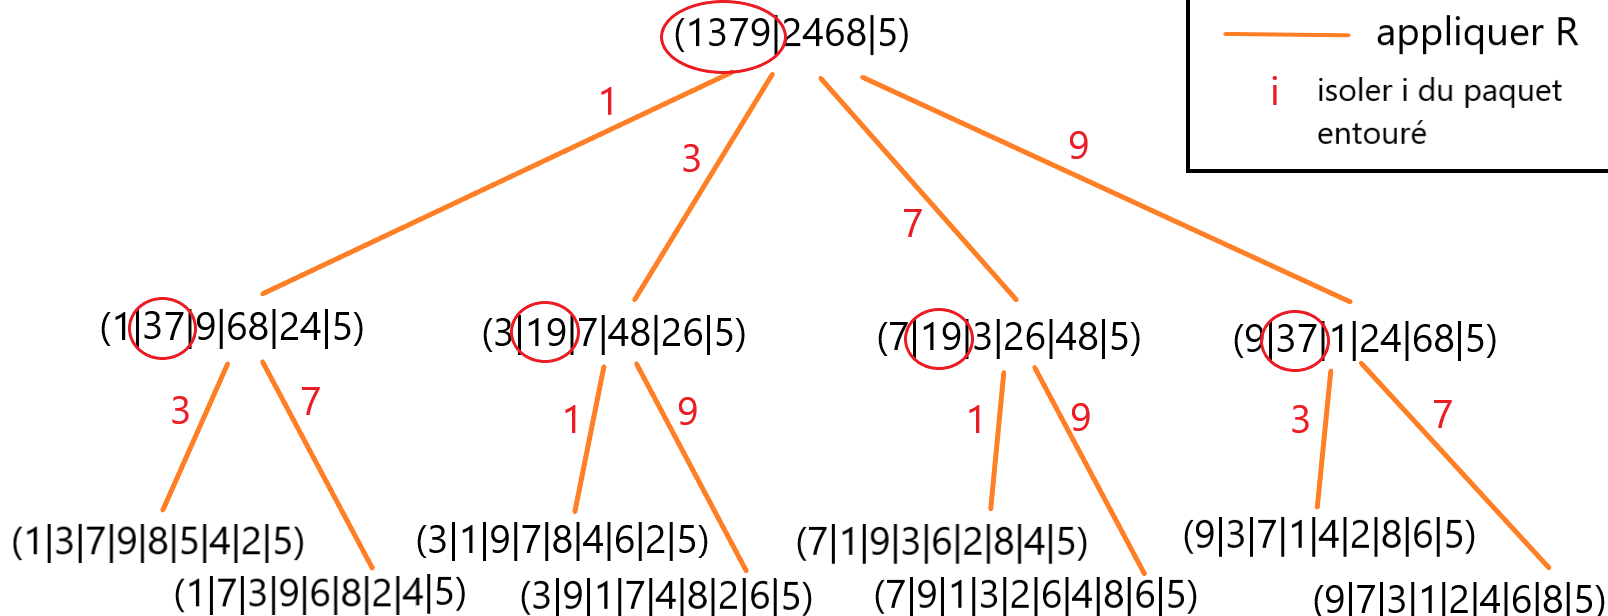
\includegraphics[width = 10cm]{search_tree}
        \caption{\label{fig:Arbre T(G)} Arbre T(G) de racine $\pi=(1\ 3\ 7\ 9\ |\ 2\ 4\ 6\ 8\ |\ 5)$}
    \end{figure}
\end{frame}

\subsection{Isomorphisme cannonique}
\begin{frame}[noframenumbering]{Relation d'ordre sur les graphes et isomorphisme cannonique}
    \underline{Ordre total $\preceq$ sur les graphes} : \newline \newline
    On pose la fonction $i:\ G\ \longmapsto i(G)$ telle que : \newline
    $\quad \bullet \ i(G)$ est la séquence binaire $(\mathds{1}_{(i,j)\in G})$ dans l'ordre lexicographique \newline
    $\quad \bullet \ G \preceq H$ si et seulement si $i(G) \leq i(H)$ en décimal
    \newline \newline
    On pose alors l'\textbf{ismorphisme cannonique de McKay} (pour le tri $\pi$):
    \begin{equation}
        \boxed{C_M(G) = max_{\preceq}\ \lbrace G^{\sigma},\ \sigma \text{ noeud terminal de T(G) de racine } \pi \rbrace }
    \end{equation}
    alors:
    \begin{equation}
        \boxed{G \cong H \text{ si et seulement si } C_M(G) = C_M(H)}
    \end{equation}
    \newline
    \underline{Exemple} : pour $\pi = (1\ |\ 3\ 7\ |\ 9\ |\ 6\ 8\ |\ 2\ 4\ |\ 5)$
    \begin{multicols}{2}
        \begin{figure}[!htb]
            \centering
            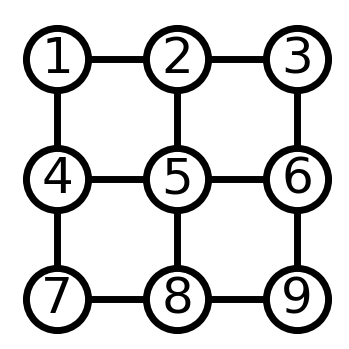
\includegraphics[width = 2.5cm]{graph_tri_equal}
            \caption{\label{fig: Graphe G}Graphe G}
        \end{figure}
        \vspace*{1cm}
        \begin{figure}[!htb]
            \centering
            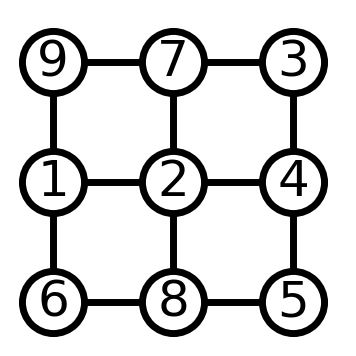
\includegraphics[width = 2.5cm]{cmg}
            \caption{\label{fig: Isomorphe G} Graphe $C_M(G)$}
        \end{figure}
    \end{multicols}
\end{frame}

\begin{frame}[allowframebreaks,noframenumbering]
    \section{Lecture PDB et génération des exemples}
    \subsection{Extraction du fichier PDB}
    \lstinputlisting[lastline=79]{extract_PDB.py}
    \subsection{Génerer les branches}
    \lstinputlisting{generer_nuage.py}
    \subsection{Modifier les protéines}
    \lstinputlisting{generer_protein.py}
    \subsection{Arbre couvrant}
    \lstinputlisting{arbre_couvrant.py}
    \subsection{Générer les graphes}
    \lstinputlisting{creer_graph.py}
    \subsection{Exemples protéines}
    \lstinputlisting[firstline=83]{extract_PDB.py}
\end{frame}
\begin{frame}[allowframebreaks,noframenumbering]
    \section{Définition des classes}  
    \subsection{Branches}
    \lstinputlisting[firstline=1,lastline=124]{cas_simple_nuage.py}
    \subsection{Graphes}
    \lstinputlisting[firstline=1,lastline=37]{graphisomorphism.py}
    \subsection{Protéines}
    \lstinputlisting[firstline=1,lastline=87]{def_protein.py}    
\end{frame}
\begin{frame}[allowframebreaks,noframenumbering]   
    \section{Isomorphisme et sous-isomorphisme}
    \subsection{Isomorphsime sur les graphes}
    \lstinputlisting[firstline=39]{graphisomorphism.py}
    \subsection{Isomorphsime sur les protéines}
    \lstinputlisting[firstline=88]{def_protein.py}
    \subsection{Sous-isomorphisme sur les protéines}
    \lstinputlisting[firstline=14,lastline=68]{subisom_prot.py}
    \subsection{Informations et temps d'exécution}
    \lstinputlisting{isom_prot.py}
    \lstinputlisting[firstline=68,lastline=73]{subisom_prot.py}
\end{frame}
\begin{frame}[allowframebreaks,noframenumbering]
    \section{Fonctions auxiliaires}
    \lstinputlisting{geometrie_et_aux.py}
\end{frame}
\begin{frame}[allowframebreaks,noframenumbering]
    \section{Calcul des coefficients}
    \lstinputlisting[firstline=126,lastline=154]{cas_simple_nuage.py}
    \lstinputlisting[firstline=91]{subisom_prot.py}
\end{frame}
\begin{frame}[allowframebreaks,noframenumbering]
    \section{Affichage}
    \subsection{Graphique complexité}
    \lstinputlisting{plot_graph_complexite_isom_brutes.py}
    \subsection{Affichage branches}
    \lstinputlisting{plot_distlines.py}
    \subsection{Affichage protéines}
    \lstinputlisting{plot_protein.py}
    \subsection{Affichage comparaison protéines}
    \lstinputlisting{plot_sub.py}
\end{frame}